% !TeX spellcheck = nl_NL
\begin{savequote}[0.55\linewidth]
	``Inspirational quote''
	\qauthor{\textasciitilde Source}
\end{savequote}

\chapter{Onderzoek}
\label{chap:onderzoek}
Zoals eerder aangehaald kan de user-perceived performance afwijken van de werkelijke performance. Dit verschil wordt voornamelijk bepaald door de interface van de applicatie. Zo ervaren gebruiker wachttijden als minder lang wanneer ze een gevoel van vooruitgang krijgen, door het gebruik van progress bars of andere visuele hints. Aangezien we bij dit onderzoek dezelfde applicatie voor beide API's gebruiken, zullen deze visuele hints de vergelijking van de user perceived performance tussen de twee diensten niet beïnvloeden. Echter biedt Linked Connections de mogelijkheid tot incrementele resultaten: nog tijdens het laden kunnen al snel eerste resultaten weergegeven worden, waardoor de gebruiker deze techniek als sneller kan ervaren, ook al duurt het langer om een gelijk aantal resultaten op te halen.

In figuur \ref{fig:expectedserviceperceivedservice} zien we de factoren die bijdragen tot de verwachting van de gebruiker en de ervaring van de gebruiker. De User Experience wordt hier tot de Service Delivery gerekend. Naast het verschil tussen de werkelijke geleverde serivce en de ervaren service, merken we ook een verschil tussen de verwachtte service en de ervaren service, in Engelstalige literatuur omschreven als een 'service quality gap'. De verwachtte service is wat de gebruiker verwacht van de applicatie, onder andere in termen van snelheid, mogelijkheden en dataverbruik. Dit correleert duidelijk met de User Experience: eerder onderzoek wees uit dat interface design, prestaties van de applicatie, batterijgebruik, kostprijs van de applicatie en connectiviteit, gebruiksersroutines en levensttijl invloed hebben op de user experience~\citep{ickin12}. In dit onderzoek zullen we ons specifiek richten op de prestaties, batterijverbruik, dataverbruik en connectiviteit.

\begin{figure}[h]
	\centering
	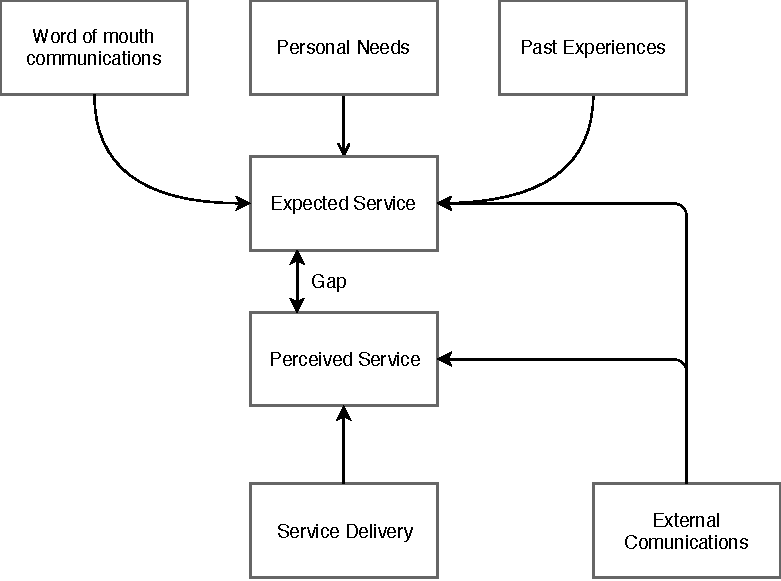
\includegraphics[width=1.00\textwidth]{expected_service.pdf}
	\caption[Factoren die bijdragen tot de verwachtingen van de gebruiker]{Factoren die bijdragen tot de verwachtingen van de gebruiker}
	\label{fig:expectedserviceperceivedservice}
\end{figure}

Tijdens dit onderzoek zullen we zowel de service delivery als perceived service proberen vergelijken tussen de twee technieken. Door deze vergelijking zullen we kunnen vaststellen of Linked Connections een betere user-perceived performance biedt, zowel absoluut als relatief ten opzichte van de werkelijke performance.

Een diepgaand onderzoek over de verwachte service valt buiten het bereik van deze masterproef. We zullen echter wel bondig de verwachtingen van gebruikers ondervragen, op vlak van dataverbruik, offline functionaliteit, en privacy, gezien deze drastisch verschillen bij Linked Connections ten opzichte van meer traditionele API's.

\section{Objectieve metingen}

Met objectieve metingen zullen we de werkelijke performance van elke API vastleggen. Ook zullen we het dataverbruik en batterijverbruik van beide technieken aan de hand van deze metingen trachten te bepalen.

Aangezien het onmogelijk is om automatisch volledige zoekopdrachten uit te voeren door de applicatie, en aangezien de benodigde tijd om te renderen een constante is die gelijk is voor alle implementaties, zal er rechtstreeks op de API implementatie getest worden, net zoals de API normaalgezien gebruikt wordt. Het uittekenen van de resultaten op het scherm is een constante, welke verwaarloosbaar klein is in vergelijking met de tijd benodigd voor het ophalen van resultaten.

Om te voorkomen dat de keuze van het geteste station of route de objectieve metingen vertekent, zullen we de opzoekingen van echte gebruikers gebruiken. Hiervoor gebruiken we de log data van api.irail.be, die publiek beschikbaar is\footnote{https://gtfs.irail.be/logs}. Door deze queries opnieuw af te spelen op de applicaties kunnen we een zo goed mogelijk beeld krijgen van de werkelijke prestaties.

Objectief zullen we proberen om volgende gegevens vast te leggen
\begin{itemize}
	\item de gemiddelde tijd om alle data van de server te halen
	\item de gemiddelde tijd tussen zoekopdracht en weergave van het eerste resultaat
	\item de gemiddelde tijd tussen zoekopdracht en weergave van het volledig resultaat
	\item de gemiddelde hoeveelheid data die verzonden en ontvangen wordt
	\item het gemiddeld processorgebruik van het toestel
	\item het gemiddeld batterijgebruik van het toestel
\end{itemize}

\section{Subjectieve metingen}

Gezien Linked Connections nog enkele belangrijke gegevens mist, zoals of een stop al dan niet afgeschaft is, en aan welk perron het voertuig zal aankomen of vertrekken, kunnen we dit systeem nog niet zelfstandig door gebruikers laten testen. Om rond deze beperking heen te werken zullen we in plaats hiervan begeleide user-tests uitvoeren met gebruikers, waarbij gebruikers gevraagd wordt om hun gebruikelijke opzoekingen te doen, per implementatie hun mening te geven, en vervolgens te bevragen welke variant hun voorkeur geniet, op vlak van snelheid, functionaliteit, en privacy.
We zullen ook zeer eenvoudig aftasten welke functionaliteit gebruikers het meest interessant vinden, zodat verder onderzoek zich hierop kan richten.

Door middel van een bevraging zullen we trachten een antwoord te vinden op volgende vragen:
\begin{itemize}
	\item Bied offline informatie een meerwaarde voor gebruikers?
	\item Hecht de gebruiker belang aan privacy bij het gebruik van routeplanning apps? Zo ja, in welke mate?
	\item Heeft de gebruiker schrik om te veel mobiele data te verbruiken?
	\item Hecht de gebruiker belang aan dataverbruik bij het gebruik van routeplanning apps?
	\item Is de gebruiker tevreden met de snelheid van zijn huidige routeplanning app?
	\item Wat is voor een gebruiker belangrijk in routeplanning apps?
	\item Is de gebruiker geïnteresseerd in routeplanning op maat? Zo ja, welke aspecten spreken hem dan aan?
	\item Is de gebruiker geïnteresseerd in offline opzoekingen?
	\item Is de gebruiker geïnteresseerd in de mogelijke snelheid die Linked Connections biedt?
	\item Is de gebruiker geïnteresseerd in de volledige privacy die Linked Connections biedt?
\end{itemize}

Door middel van user-testing zullen we proberen om ook deze vragen te beantwoorden:
\begin{itemize}
	\item Ervaart de gebruiker een app die lokaal Linked Connections gebruikt als sneller dan een app die gebruik maakt van een RPC API?
	\item Ervaart de gebruiker een app die lokaal Linked Connections gebruikt als sneller dan zijn huidige app?
\end{itemize}

Om een antwoord op bovenstaande vragen te vinden, werd een enquete opgebouwd. Deze exacte vraagsteling voor deze enquete is terug te vinden in bijlage \ref{appendix:enquete}.